\documentclass[twocolumn]{aastex63}

\bibliographystyle{aasjournal}
\usepackage{subfigure}
\usepackage{url}
\usepackage{hyperref}
%\usepackage{datetime}
\usepackage{longtable}
\usepackage{natbib}
\usepackage{amsmath}
\usepackage{listings}
\usepackage[normalem]{ulem}
\usepackage{bm}
\usepackage{comment}
% additions for ease of tabling
\usepackage{array}
\newcolumntype{P}[1]{>{\centering\arraybackslash}p{#1}}
\newcolumntype{M}[1]{>{\centering\arraybackslash}m{#1}}
% colors
%\usepackage[usenames, dvipsnames]{color}

%\usepackage{pdflscape}
\usepackage{xcolor, fontawesome}
\definecolor{twitterblue}{RGB}{64,153,255}
\newcommand{\twitter}[1]{\href{https://twitter.com/#1 }{\textcolor{twitterblue}{\faTwitter}\,\tt \textcolor{twitterblue}{@#1}}}

\definecolor{Code}{rgb}{0,0,0}
\definecolor{Decorators}{rgb}{0.5,0.5,0.5}
\definecolor{Numbers}{rgb}{0.5,0,0}
\definecolor{MatchingBrackets}{rgb}{0.25,0.5,0.5}
\definecolor{Keywords}{rgb}{1,0,0}
\definecolor{self}{rgb}{0,0,0}
\definecolor{Strings}{rgb}{0,0.63,0}
\definecolor{Comments}{rgb}{0,0.63,1}
\definecolor{Backquotes}{rgb}{0,0,0}
\definecolor{Classname}{rgb}{0,0,0}
\definecolor{FunctionName}{rgb}{0,0,0}
\definecolor{Operators}{rgb}{0,0,0}
\definecolor{Background}{rgb}{0.98,0.98,0.98}
\definecolor{Booleans}{rgb}{0.572,0,0.572}
\definecolor{BuiltinFunction}{rgb}{0.572,0,0.572}
\definecolor{BuiltinConstant}{rgb}{0.572,0,0.572}
\definecolor{Asterisk}{rgb}{0.670,0,1}

\lstdefinelanguage{Python}{
    	numbers=left,
    	numberstyle=\footnotesize,
    	numbersep=7pt,
    	xleftmargin=1.26em,
    	framextopmargin=2em,
    	framexbottommargin=2em,
    	showspaces=false,
    	showtabs=false,
    	showstringspaces=false,
    	frame=l,
    	tabsize=4,
    	stepnumber=1,
	% Basic
	basicstyle=\small\ttfamily,
    	backgroundcolor=\color{Background},
%    	breaklines=True,
%    	postbreak=\mbox{\textcolor{red}{$\hookrightarrow$}\space},
	% Comments
%	commentstyle=\color{green}\ttfamily,
	% Strings
%    	stringstyle=\ttfamily\color{Strings},
%    	morecomment=[s][\color{Strings}]{'}{'}, 
%    	stringstyle=\ttfamily\color{Comments},
%    	morecomment=[s][\color{Comments}]{\#}{\#}, 			
	% Keywords
	stringstyle=\ttfamily\color{Strings},
	morekeywords={import,from,class,def,while,if,in,elif,else,not,or,print,break,continue,return,access,as,except,exec,finally,global,import,lambda,pass,print,raise,try,assert},
    	keywordstyle={\color{Keywords}\bfseries}, 
    %	morekeywords={[2]True,False,None},
    %	keywordstyle={[2]\color{BuiltinConstant}\slshape},
	otherkeywords={[2]*},
	keywordstyle={[2]\color{Asterisk}},
%	emph={self},
%	emphstyle={\color{self}\slshape}	
}

\usepackage{color}

\newcommand{\ron}{\color{red}} 
\newcommand{\bon}{\color{blue}} 
\newcommand{\gon}{\color{green}} 
\newcommand{\coff}{\color{black}\,}
\newcommand{\shrug}{\texttt{\raisebox{0.75em}{\char`\_}\char`\\\char`\_\kern-0.5ex(\kern-0.25ex\raisebox{0.25ex}{\rotatebox{45}{\raisebox{-.75ex}"\kern-1.5ex\rotatebox{-90})}}\kern-0.5ex)\kern-0.5ex\char`\_/\raisebox{0.75em}{\char`\_}}}


\newcommand{\rprs}{{$R_p/R_{\star}$}}

\newcommand{\eg}{{\it e.g.}}
\newcommand{\ie}{{\it i.e.}}
\newcommand{\kep}{{\it Kepler}}
\newcommand{\kt}{{\it K2}}
\newcommand{\tess}{{\it TESS}}
\newcommand{\ffis}{Full-Frame Images}
\newcommand{\fulltess}{{\it Transiting Exoplanet Survey Satellite}}
\newcommand{\Gaia}{{\it Gaia}}
\newcommand{\spitz}{{\it Spitzer}}
\newcommand{\vsini}{{$V \sin i$}}
\newcommand{\teff}{$T_{ eff}$}
\newcommand{\kms}{{km\,s$^{-1}$}}
\newcommand{\gcc}{{g\,cm$^{-3}$}}
\newcommand{\rstar}{{$R_\star$}}
\newcommand{\rhostar}{{$\rho_\star$}}
\newcommand{\mearth}{{M$_\oplus$}}
\newcommand{\rearth}{{R$_\oplus$}}
\newcommand{\rsun}{{R$_\odot$}}
\newcommand{\msun}{{M$_\odot$}}
\newcommand{\mjup}{{M$_\textrm{Jup}$}}
\newcommand{\rjup}{{R$_\textrm{Jup}$}}

\newcommand{\eleanor}{\texttt{eleanor}}

\newcommand{\mstar}{{$M_\star$}}
\newcommand{\logg}{{log(g)}}
\newcommand{\mh}{{[M/H]}~}
\newcommand{\feh}{{[Fe/H]}~}
%\newcommand{\h2ok2}{{$ H_2O-K2$}}

\newcommand{\todo}[3]{{\color{#2} \emph{#1} TO DO: #3}}
\newcommand{\mkntodo}[1]{\todo{ADINA}{cyan}{#1}}
\newcommand{\btmtodo}[1]{\todo{BEN}{blue}{#1}}
\newcommand{\anytodo}[1]{\todo{ANYONE}{green}{#1}}

\newcommand{\comm}[1]{{\color{cyan}{#1}}}

\newcommand{\Sph}{{$S_{\textrm{ph}}$}}
\newcommand{\RHK}{{$R'_{\textrm{HK}}$}}

\newcommand{\unsw}{School of Physics, University of New South Wales, Sydney, NSW 2052, Australia}
\newcommand{\chicago}{Department of Astronomy and Astrophysics, University of
Chicago, 5640 S. Ellis Ave, Chicago, IL 60637, USA}

\newcommand{\grfp}{NSF Graduate Research Fellow}

\newcommand{\flatiron}{Center for Computational Astrophysics, Flatiron Institute, 162 Fifth Ave, New York, NY 10010, USA}

\newcommand{\dtm}{Department of Terrestrial Magnetism, Carnegie Institute of Washington, Washington, DC 20015, USA}

\newcommand{\carnegie}{Observatories of the Carnegie Institution for Science, 813 Santa Barbara St., Pasadena, CA 91101}

\newcommand{\princeton}{Department of Astrophysical Sciences, Princeton University, 4 Ivy Lane, Princeton, NJ 08544, USA}

\newcommand{\ames}{NASA Ames Research Center, Moffett Field, CA 94035, USA}


%\submitted{for May 2, 2016}

\begin{document}
\title{The Young Planet DS Tuc Ab has a Low Obliquity}

\shorttitle{DS Tuc Ab has a Low Obliquity} 
\shortauthors{Montet et al.}


\author[0000-0001-7516-8308]{Benjamin~T.~Montet}
\affiliation{\unsw}
\affiliation{\chicago}

\author[0000-0002-9464-8101]{Adina~D.~Feinstein}
\altaffiliation{\grfp}
\affiliation{\chicago}

\author{Rodrigo Luger}
\affiliation{\flatiron}

\author{Megan E. Bedell}
\affiliation{\flatiron}

\author{Johanna K. Teske}
\altaffiliation{Hubble Fellow}
\affiliation{\carnegie}
\affiliation{\dtm}

\author{Sharon Xuesong Wang}
\affiliation{\dtm}

\author{R. Paul Butler}
\affiliation{\dtm}

\author{Erin Flowers}
\affiliation{\princeton}

\author{Michael A. Gully-Santiago}
\affiliation{\ames}

\author{Stephen A. Shectman}
\affiliation{\carnegie}

\author{Jeffrey D. Crane}
\affiliation{\carnegie}

\author{Ian B. Thompson}
\affiliation{\carnegie}




%\correspondingauthor{Benjamin~T.~Montet; \twitter{benmontet}}
\email{b.montet@unsw.edu.au}

%@arxiver{f8a.pdf,f5.pdf,f2b.pdf}
%\date{\today, \currenttime}

\begin{abstract}

The abundance of short-period planetary systems with high obliquities is often taken as evidence that scattering processes play important roles in the formation and evolution of these systems.
More recent studies have suggested that wide binary companions can tilt protoplanetary disks, inducing a high obliquity on planets that form through smooth processes like disk migration.
\object{DS Tuc Ab}, a planet in the 45 Myr Tucana-Horologium association, likely traces its now-dissipated protoplanetary disk, enabling us to test these theories of disk physics. 
Here, we report on Rossiter-McLaughlin observations of one transit of DS Tuc Ab with the Planet Finder Spectrograph on the Magellan Clay Telescope at Las Campanas Observatory. 
We confirm the previously statistically validated planet by modeling the planet transit and stellar activity signals simultaneously, finding its obliquity to be low: $\psi = 12 \pm 13$ degrees. 
This is the youngest planet to be observed using this technique; we provide a discussion on best practices to accurately measure the observed signal of similar young planets.
\end{abstract}

\keywords{Exoplanets (498), Exoplanet dynamics (490), High resolution spectroscopy (2096), Starspots (1572)}


 
\section{Introduction} \label{sec:intro}

Planet formation is poorly understood \citep[e.g.][]{Morbidelli16}. 
Each discovered planetary system represents an outcome of the planet formation process, and therefore provides an opportunity to learn about how different planets form in different environments. 
However, each observed present-day system is not a pure laboratory: over billions of years, planet-planet and planet-star gravitational interactions can scatter, torque, migrate, or otherwise perturb orbits, distancing planetary systems from their formation state \citep{Kozai62, Lidov62, Fabrycky07, Chatterjee08}. 
This picture is complicated by the fact that in many cases, stellar ages are very poorly known \citep[e.g.][]{Barnes07, Soderblom10}.

The origins of hot Jupiters are still unclear \citep{Dawson18}.
Kozai-Lidov cycles and tidal friction are often invoked to explain the formation of hot Jupiters \citep{Fabrycky07}, but smooth disk migration provides a reasonable alternative in many cases \citep{Ida08}. 
It is possible that multiple channels are required in order to explain all of the observed systems: \citet{Nelson17} analyze data from the HAT and WASP exoplanet surveys and find the data can be well-fit by a model in which $\sim85\%$ of hot Jupiters are formed through high-eccentricity migration and $\sim15\%$ through disk migration.

Planets in young clusters are valuable resources to provide clean test cases for planet formation. 
Dynamical interactions like the Kozai-Lidov effect can, depending on the system architecture, occur over hundreds of millions or billions of years \citep{Montet15c, Naoz16}. 
For systems with younger ages, we can rule out certain dynamical interactions, meaning it is likely that the orbit of the planet traces the orbit of the now-dissipated disk. 

Therefore, by measuring the obliquity of the orbits of young planets relative to the spin of their host stars, we are tracing the obliquity of their disks. 
Observing a population of these systems will allow us to understand statistical disk properties. 
Alignment of planetary systems and their host stars is often taken as evidence in favor of smooth migration processes. \btmtodo{cite papers here}. 
However, \btmtodo{Batygin citation} suggest wide binary companions or nearby stars in the birth cluster can torque disks to random inclinations over the lifetime of the disk. With a statistical sample of the obliquities of young planets, we can test this hypothesis.

Such a survey is limited by the small number of planetary systems around young stars. There are only a handful of planets known to be younger than 100 Myr, identified by their membership in young moving groups or star forming regions \btmtodo{citep David19, Mann, others}.

Recently, data from the Transiting Exoplanet Survey Satellite \citep{Ricker14} were used to identify a planet with an orbital period of 8.14 days around the star \object{DS Tuc A} \citep{Benatti19, Newton19}. 
DS Tuc is a member of the Tucana-Horologium (Tuc-Hor) assocation, which has an age of approximately 45 Myr \btmtodo{cite!}. 
DS Tuc itself is a binary with a projected separation of \btmtodo{AU}. 
From \citet{Holman97}, the timescale for Kozai-Lidov interactions is
\begin{equation}
    \tau \approx P_\textrm{planet} \frac{M_\star}{M_\textrm{pert}} \bigg(\frac{a_\textrm{pert}}{a_\textrm{planet}}\bigg)^3 (1-e^2_\textrm{pert})^{3/2},
\label{eq:timescale}
\end{equation}
where $P_\textrm{planet}$ is the the orbital period of a planet with orbital semimajor axis  $a_\textrm{planet}$ about a host of mass $M_\star$, $M_\textrm{pert}$ is the
mass of the perturbing star, and $a_\textrm{pert}$ and $e_\textrm{pert}$ the semimajor axis and eccentricity of the outer object's orbit around the host star/planet system.

From the orbital parameters in \citet{Newton19}, ${M_\star}/{M_\textrm{pert}} \approx 1.2$, ${a_\textrm{pert}}/{a_\textrm{planet}} \approx 2000$, and $(1-e^2_\textrm{pert})^{3/2} \approx 0.5$, so the timescale $\tau$ from Equation \ref{eq:timescale} is more than 100 Myr. 

Therefore, this planet likely traces the orientation of the now-dissipated protoplanetary disk. 
Measuring the obliquity of the planet relative to the star thus enables us to test theories of disk torqing.
We can measure the obliquity between the spin of the star and the orbit of the planet through the Rossiter-McLaughlin effect, in which an apparent redshift and blueshift in the radial velocity of the star are observed as a transiting planet occults the blueshifted and redshifted hemispheres of the rotating star, respectively \citep{Rossiter24, McLaughlin24}.
DS Tuc Ab is the youngest known planet for which such an observation has been attempted, providing us the nearest test case to an undissipated disk yet acheivable.


The rest of this paper is organized as follows:
In Section \ref{sec:obs} we describe the observations.
In Section \ref{sec:analysis} we describe our data analysis.
In Section \ref{sec:results} we present our results.
In Section \ref{sec:discussion}, we discuss best practices for future similar observations of young stars and potential confounding factors, as well as future work.


\section{Observations}
\label{sec:obs}

We obtained data with the Planet Finder Spectrograph (PFS) on the Magellan Clay Telescope \citep{Crane06, Crane08, Crane10}. 
On \btmtodo{date} from \btmtodo{time} to \btmtodo{time} we obtained \btmtodo{number} of measurements of the RV of DS Tuc A. The transit duration is 190 minutes, meaning approximately 50\% of the data were obtained in transit while the other half provide information about the out-of-transit RV baseline. Each exposure was 360 seconds in length and was taken with the \btmtodo{slit} slit, which provides a resolution $R \approx$ \btmtodo{number} per btmtodo{pixel or resolution element?}. All observations were taken with the iodine cell in place \citep{Marcy92}, which imprints a series of narrow lines at known wavelengths to measure the instrument point spread function and wavelength solution at each epoch.

\todo{pfs team}{red}{Is there anything else you would like us to include?}

To characterize the stellar activity-induced variations, we also obtained \btmtodo{more}
These observations had exposure lengths varying from 360 to 600 seconds under variable sky conditions, with the goal of achieving a similar SNR in each of these spectra as during the night of the transit.

We also collected a template spectrum of DS Tuc A immediately after the transit observations. 
This spectrum, obtained under similar conditions and with the same slit but without the iodine cell in the light path, is used in the pipeline RV modeling.
All observations were then analyzed using the standard PFS pipeline \citep{Butler96}, which divides the spectrum into 2\AA\ chunks and fits each chunk independently.
The resultant RV is the weighted mean of the RVs of each chunk, and the provided uncertainty is the standard deviation of these velocities.

\btmtodo{Paragraph here about what RVs are included in the modeling}

The resultant RVs are given in Table \ref{tab:data} and displayed in Figure \ref{fig:data}.


\startlongtable
\begin{deluxetable*}{lcccc}
\tablecaption{Derived RVs for DS Tuc A. \label{tab:data}}
\tablehead{
\colhead{Time} & \colhead{RV} & \colhead{Uncertainty} & \colhead{$S_{HK}$} & \colhead{H$\alpha$} \\
\colhead{(BJD)} & \colhead{(m s$^{-1}$)} & \colhead{(m s$^{-1}$)} & {} & {}
}
\startdata
2458706.55618 &  -10.84 & 4.83 &  0.5826 & 0.05566 \\
2458706.56101 &  -14.13 & 4.14 &  0.5735 & 0.05596 \\
2458706.56592 &  -11.80 & 4.45 &  0.5679 & 0.05615 \\
2458706.57080 &  -23.17 & 4.59 &  0.5712 & 0.05566 \\
2458706.57570 &  -20.68 & 3.82 &  0.5727 & 0.05597 \\
2458706.58047 &  -24.58 & 4.33 &  0.5771 & 0.05603 \\
2458706.58537 &  -23.59 & 4.01 &  0.5737 & 0.05593 \\
2458706.59023 &  -26.70 & 4.58 &  0.5809 & 0.05613 \\
2458706.59529 &  -18.26 & 4.61 &  0.5849 & 0.05630 \\
2458706.60010 &  -17.40 & 4.56 &  0.5887 & 0.05648 \\
2458706.60506 &  -26.49 & 4.97 &  0.5993 & 0.05594 \\
2458706.60996 &    9.87 & 4.96 &  0.5900 & 0.05670 \\
2458706.61486 &   20.74 & 4.41 &  0.5936 & 0.05597 \\
2458706.61966 &   12.43 & 4.68 &  0.5992 & 0.05641 \\
2458706.62472 &   14.68 & 4.59 &  0.5853 & 0.05667 \\
2458706.62965 &   22.34 & 4.90 &  0.6046 & 0.05718 \\
2458706.63939 &   26.89 & 4.26 &  0.5839 & 0.05625 \\
2458706.64420 &   26.72 & 4.79 &  0.5985 & 0.05671 \\
2458706.65419 &   15.13 & 4.97 &  0.5898 & 0.05628 \\
2458706.65893 &    8.84 & 3.88 &  0.5716 & 0.05611 \\
2458706.66370 &    4.60 & 3.64 &  0.5712 & 0.05614 \\
2458706.66866 &   -4.96 & 4.21 &  0.5858 & 0.05610 \\
2458706.67356 &  -10.62 & 4.09 &  0.5781 & 0.05598 \\
2458706.67856 &  -21.84 & 3.79 &  0.5755 & 0.05600 \\
2458706.68325 &  -29.88 & 3.91 &  0.5752 & 0.05585 \\
2458706.68844 &  -45.36 & 4.55 &  0.5793 & 0.05599 \\
2458706.69319 &  -42.99 & 3.89 &  0.5684 & 0.05592 \\
2458706.69809 &  -32.38 & 4.02 &  0.5645 & 0.05529 \\
2458706.70304 &  -43.37 & 3.90 &  0.5606 & 0.05518 \\
2458706.70783 &  -35.81 & 3.98 &  0.5680 & 0.05540 \\
2458706.71273 &  -38.21 & 3.85 &  0.5670 & 0.05539 \\
2458706.71765 &  -46.83 & 3.91 &  0.5659 & 0.05522 \\
2458706.72256 &  -33.74 & 4.06 &  0.5646 & 0.05535 \\
2458706.72746 &  -26.33 & 4.21 &  0.5659 & 0.05535 \\
2458706.73235 &    4.43 & 3.97 &  0.5588 & 0.05521 \\
2458706.73731 &    9.93 & 3.52 &  0.5567 & 0.05513 \\
2458706.74210 &    6.50 & 3.89 &  0.5596 & 0.05489 \\
2458706.74700 &    8.13 & 3.74 &  0.5571 & 0.05511 \\
2458706.75197 &    8.98 & 3.97 &  0.5574 & 0.05508 \\
2458706.75683 &   23.30 & 4.15 &  0.5646 & 0.05516 \\
2458706.76179 &   13.34 & 3.98 &  0.5647 & 0.05524 \\
2458706.76657 &   12.16 & 4.56 &  0.5607 & 0.05499 \\
2458706.77163 &   13.26 & 4.39 &  0.5632 & 0.05460 \\
2458706.77643 &   13.52 & 4.49 &  0.5623 & 0.05483 \\
2458706.78139 &   14.45 & 4.47 &  0.5607 & 0.05495 \\
2458706.78620 &   25.45 & 4.27 &  0.5590 & 0.05460 \\
2458706.79111 &    0.00 & 4.46 &  0.5577 & 0.05445 \\
2458706.79602 &   34.67 & 4.21 &  0.5524 & 0.05464 \\
2458706.80090 &   31.51 & 4.25 &  0.5585 & 0.05452 \\ 
\hline
2458716.59155 &  100.30 & 5.84 & -- & -- \\
2458716.72215 &  105.19 & 6.25 & -- & -- \\
2458717.62611 &  146.51 & 8.11 & -- & -- \\
2458717.77760 &  -71.01 & 7.04 & -- & -- \\
2458737.72011 &  199.55 & 8.73 & -- & -- \\
2458737.80174 &  131.10 & 8.98 & -- & -- \\
2458738.67055 &  -76.18 & 7.18 & -- & -- \\
2458738.76341 &  -79.52 & 7.87 & -- & -- \\
2458739.65311 &   67.24 & 7.91 & -- & -- \\
2458739.77091 &  135.17 & 8.23 & -- & -- \\
2458740.65811 &   66.63 & 7.77 & -- & -- \\
2458740.75524 &   22.49 & 7.56 & -- & -- \\
\enddata
\end{deluxetable*}

\begin{figure}[!tbh]
  \begin{center}
    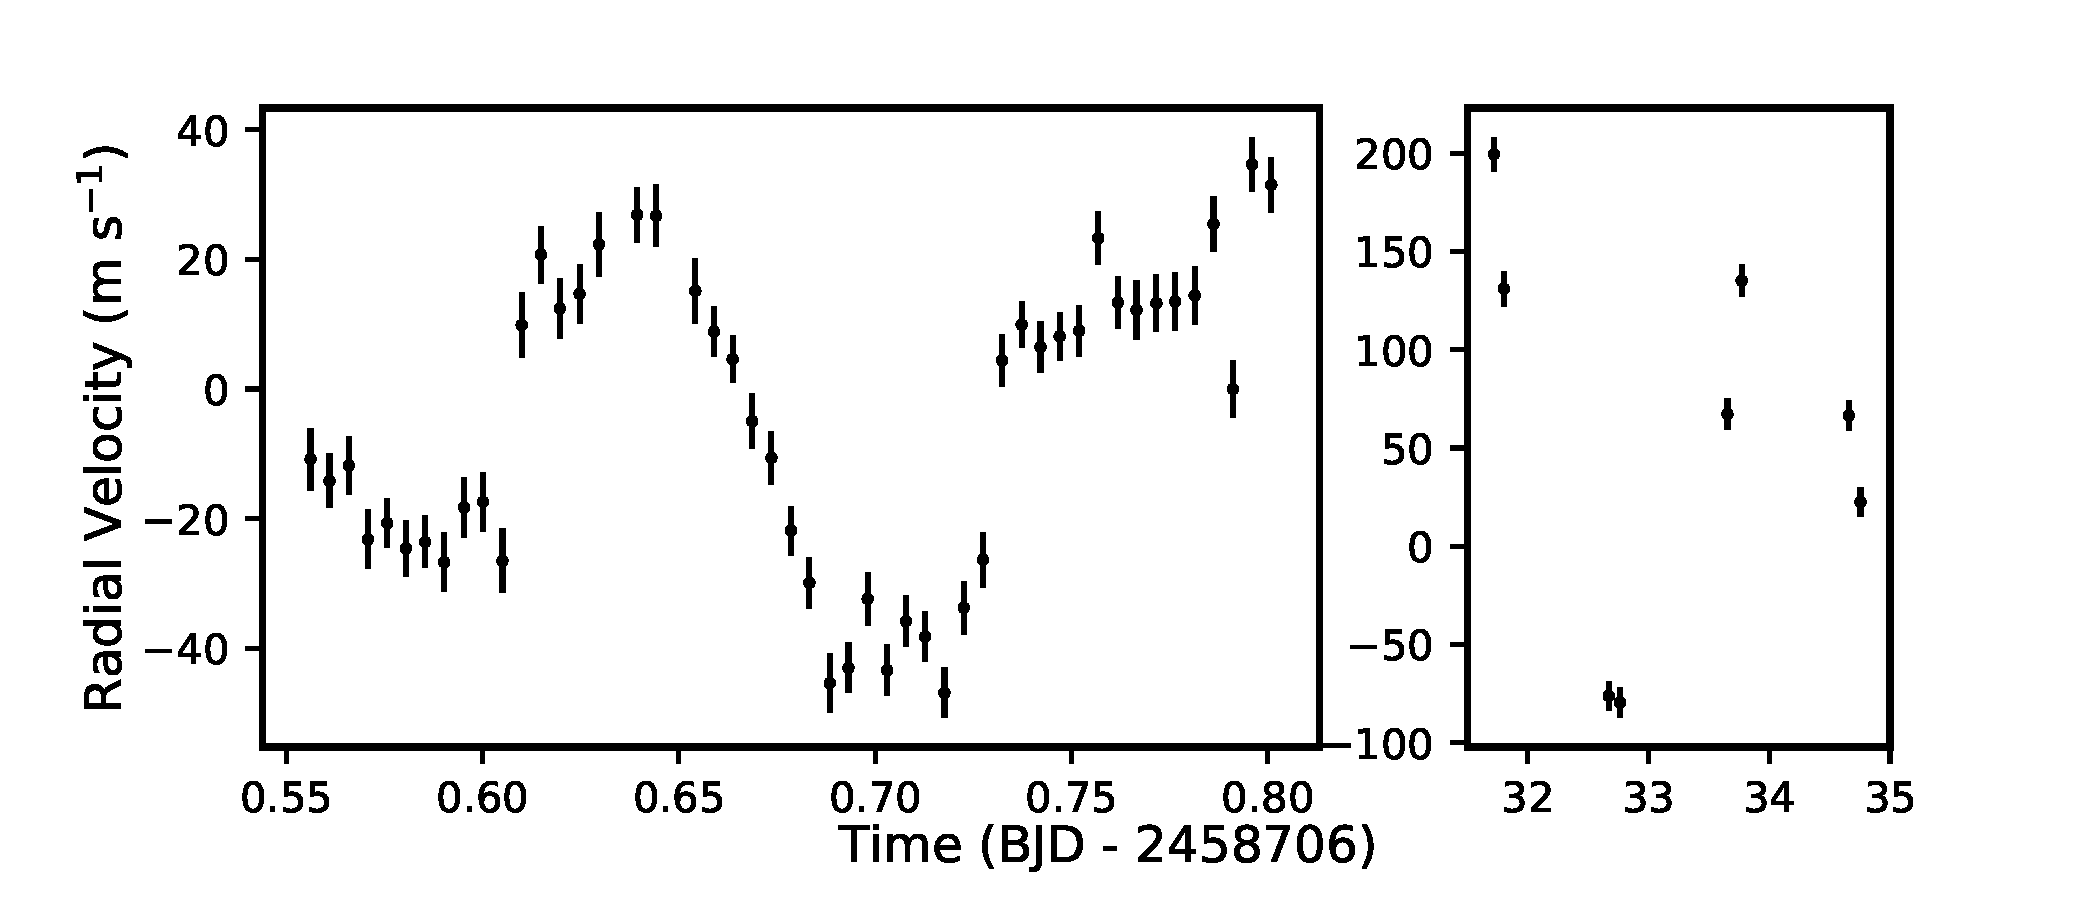
\includegraphics[width=0.5\textwidth, trim={0cm 0.0cm 0cm 0cm}, clip=true]{../figures/all_data.pdf}
   \end{center}
  \caption{RV time series for (left) the observed transit and (right) a timespan covering approximately one stellar rotation period. Note the different vertical scalings on each subplot. The Rossiter-McLaughlin signal is easily detectable, occurring over a significantly different timescale than the rotationally-induced variability signal.}
  \label{fig:data}
\end{figure}



\section{Data analysis}
\label{sec:analysis}

We model the inferred radial velocities with version 1.0.0.dev3 of the \textit{starry} package of \citet{Luger19}. 
\textit{starry} models the star as a series of spherical harmonics. 
\todo{RODRIGO}{red}{please put a couple sentences about starry here, especially in how it does the R-M signal behind the scenes.}

\btmtodo{Mention that we force circular orbits}

\subsection{Model}

Over the six hours of the transit, the apparent radial velocity of the star increases by \btmtodo{number} m s$^{-1}$. 
In Section \ref{sec:trend} we argue this trend is due to stellar activity rather than an additional planet.
To understand the obliquity of the transiting planet, for now we are only concerned with appropriately modeling this signal.
We attempt to model this signal through multiple approaches.
We use low-order polynomials, up to the third degree, to fit the extra variability during the night of the transit. 
We also build a stellar activity model by fitting a function that is a linear sum of the observed $H\alpha$ and calcium $S_{HK}$ measurements during the night, which are correlated with the observed RV.
Finally, we also fit \textit{starry} models of a single starspot in time. The spot is modeled as a Gaussian darker region on the surface of the star; we allow the spot's size, contrast, and location to vary as we fit both signals.

In each case, we then build a model that is the sum of the R-M signal and the stellar activity signal at each cadence, such that
With three separate models, we can use the inferred likelihood to compare the abilities of these activity models to fit the data. 
It also gives us the opportunity to verify that the resultant obliquity measurement does not depend on the specific prescription of the stellar activity signal.

\btmtodo{this whole section uses the term `model' too much}



\subsection{Likelihood Function}

To compare the data to our model, we need to write down a likelihood function. 
Each observation has an associated uncertainty, calculated as the \todo{pfs team}{red}{how exactly are the uncertainties calculated in the PFS pipeline?}
For this young and active star, this likelihood may not represent the true uncertainty in the measured RV at each epoch. 
For example, occultations of small spots across the surface of the star could cause the observed RV to vary from epoch to epoch. 
Additionally, stellar flares would have characteristic timescales similar to a single exposure and could impact the observed RV if a significant amount of emission from the star was ejected from the surface of the star with considerable velocity \btmtodo{cite here}.

We test multiple likelihood functions with the same form.
First, we assume a model that is the sum of two Gaussians with the same mean but different variance. 
Under this model, each data point has some probability $q$ of being a ``good'' data point drawn from a relatively narrow distribution. This distribution is a combination of the PFS pipeline uncertainty and an additional jitter term, added in quadrature. 
Each data point also has a probability $1-q$ of being drawn from a much broader distribution. We allow the width of both Gaussian distributions to vary in our fitting procedure. 
Additionally, $q$ is a free parameter: if the data were well-modeled by a single Gaussian, we would find the posterior distribution on $q$ to be consistent with zero.

These two Gaussians do not need to have the same mean. 
The surface of the star, as a rapidly rotating G dwarf, is likely dominated by dark starspots rather than bright faculae \citep{Montet17}. 
Each dark spot will have the effect of inducing a signal with roughly the same shape as the R-M effect for an aligned system: as the spot occults the blueshifted hemisphere of the star, it will induce an apparent redshift and vice versa.
As a planet occults a spot then, just as this phenomenon produces a brief brightening in a transit light curve \btmtodo{cite spot crossing papers here} a spot-crossing event would cause a temporary decrease in the magnitude of the Rossiter-McLaughlin signal. 
We then allow for the broader Gaussian in our mixture model to be offset by some factor which is directly proportional to the magnitude of the R-M signal at that epoch. The mean of our second Gaussian is then
\begin{equation}
\mu_2 = \alpha (RV_{RM}).
\end{equation}
When $\alpha = 1$, the means of the two Gaussians overlap precisely, leaving us with a standard mixture model as might be expected if the extra variability was not related to starspots. 
We test both the case where $\alpha$ is set equal to 1, and also allowed to vary as a free parameter.

Our full likelihood function is then
\begin{equation}
\mathcal{L} \propto 1	
\end{equation}
\btmtodo{write this out}
where \btmtodo{stuff equals stuff}

\subsection{Fitting}





Don't forget to mention our priors here!

Something in the models subsubsection about Halpha being less noisy than Shk for this star. Probably because of the wavelengths we're dealing with?

Gee, MCMC sure is cool.


\section{Results}
\label{sec:results}

$10 \pm 10$ degrees, roughly.


\begin{deluxetable*}{lccc}[!ht]
\tablecaption{Inferred transit parameters \label{tab:results}}
\tablehead{
\colhead{} & \colhead{Polynomial Model} & \colhead{Stellar Activity Correlation Model} & \colhead{Starspot Fit} 
}
\startdata
\vsini\ (km s$^{-1}$) & $19.6 \pm 1.5$ & $20.0 \pm 1.6$ & $19.4 \pm 1.5$ \\
$R_p/R_\star$ & $0.059 \pm 0.002$ & $0.060 \pm 0.003$ & $0.059 \pm 0.002$ \\
$t_0$ ($\textrm{BJD}-2457000$) & $1706.6654 \pm 0.0010$ & $1706.6653 \pm 0.0018$ &
              $1706.6655 \pm 0.0012$\\
$b$ & $0.18 \pm 0.11$ & $0.17 \pm 0.13$ & $0.18 \pm 0.12$ \\
$a/$\rstar & $20.8 \pm 0.7$ & $21.2 \pm 1.1$ & $20.9 \pm 0.8$ \\
Obliquity (deg) & $14 \pm 11$ & $5 \pm 11$ & $12 \pm 13$ \\
Obliquity (deg), $q=1$ & $12 \pm 11$ & $13 \pm 6$ & $7 \pm 12$ \\
Obliquity (deg), $\alpha = 1$ & $14 \pm 13$ & $3 \pm 11$ & $8 \pm 15$ \\
\hline
Spot Amplitude & - & - & $0.019 \pm 0.005$ \\
Spot Size (\rstar) & - & - & $0.055 \pm 0.023$ \\
Spot Longitude\tablenotemark{a} (deg) & - & - & $26 \pm 4$ \\
Spot Latitude\tablenotemark{a} (deg) & - & - & $28 \pm 8$ \\
\hline
jitter 1 (m s$^{-1}$) & $1.8 \pm 0.9$ & $1.5 \pm 0.9$ & $1.8 \pm 0.9$ \\
jitter 2 (m s$^{-1}$) & $8.8 \pm 4.4$ & $11.9 \pm 3.0$ & $9.3 \pm 5.4$ \\
$q$ & $0.54 \pm 0.24$ & $0.32 \pm 0.17$ & $0.58 \pm 0.24$ \\
$\alpha$ & $0.88 \pm 0.08$ & $0.88 \pm 0.11$ & $0.85 \pm 0.15$ \\
\hline
$\log \mathcal{L}_\textrm{max}$ & $-162.2$ & $-178.3$ & $-162.1$ \\
Bayes' Factor & 0.83 & $9.1 \times 10^{-8} $ & 1.0
\enddata
\tablenotetext{a}{Defined at $\textrm{BJD}-2457000 = 1706.5$}
\end{deluxetable*}


\begin{figure}[!tbh]
  \begin{center}
    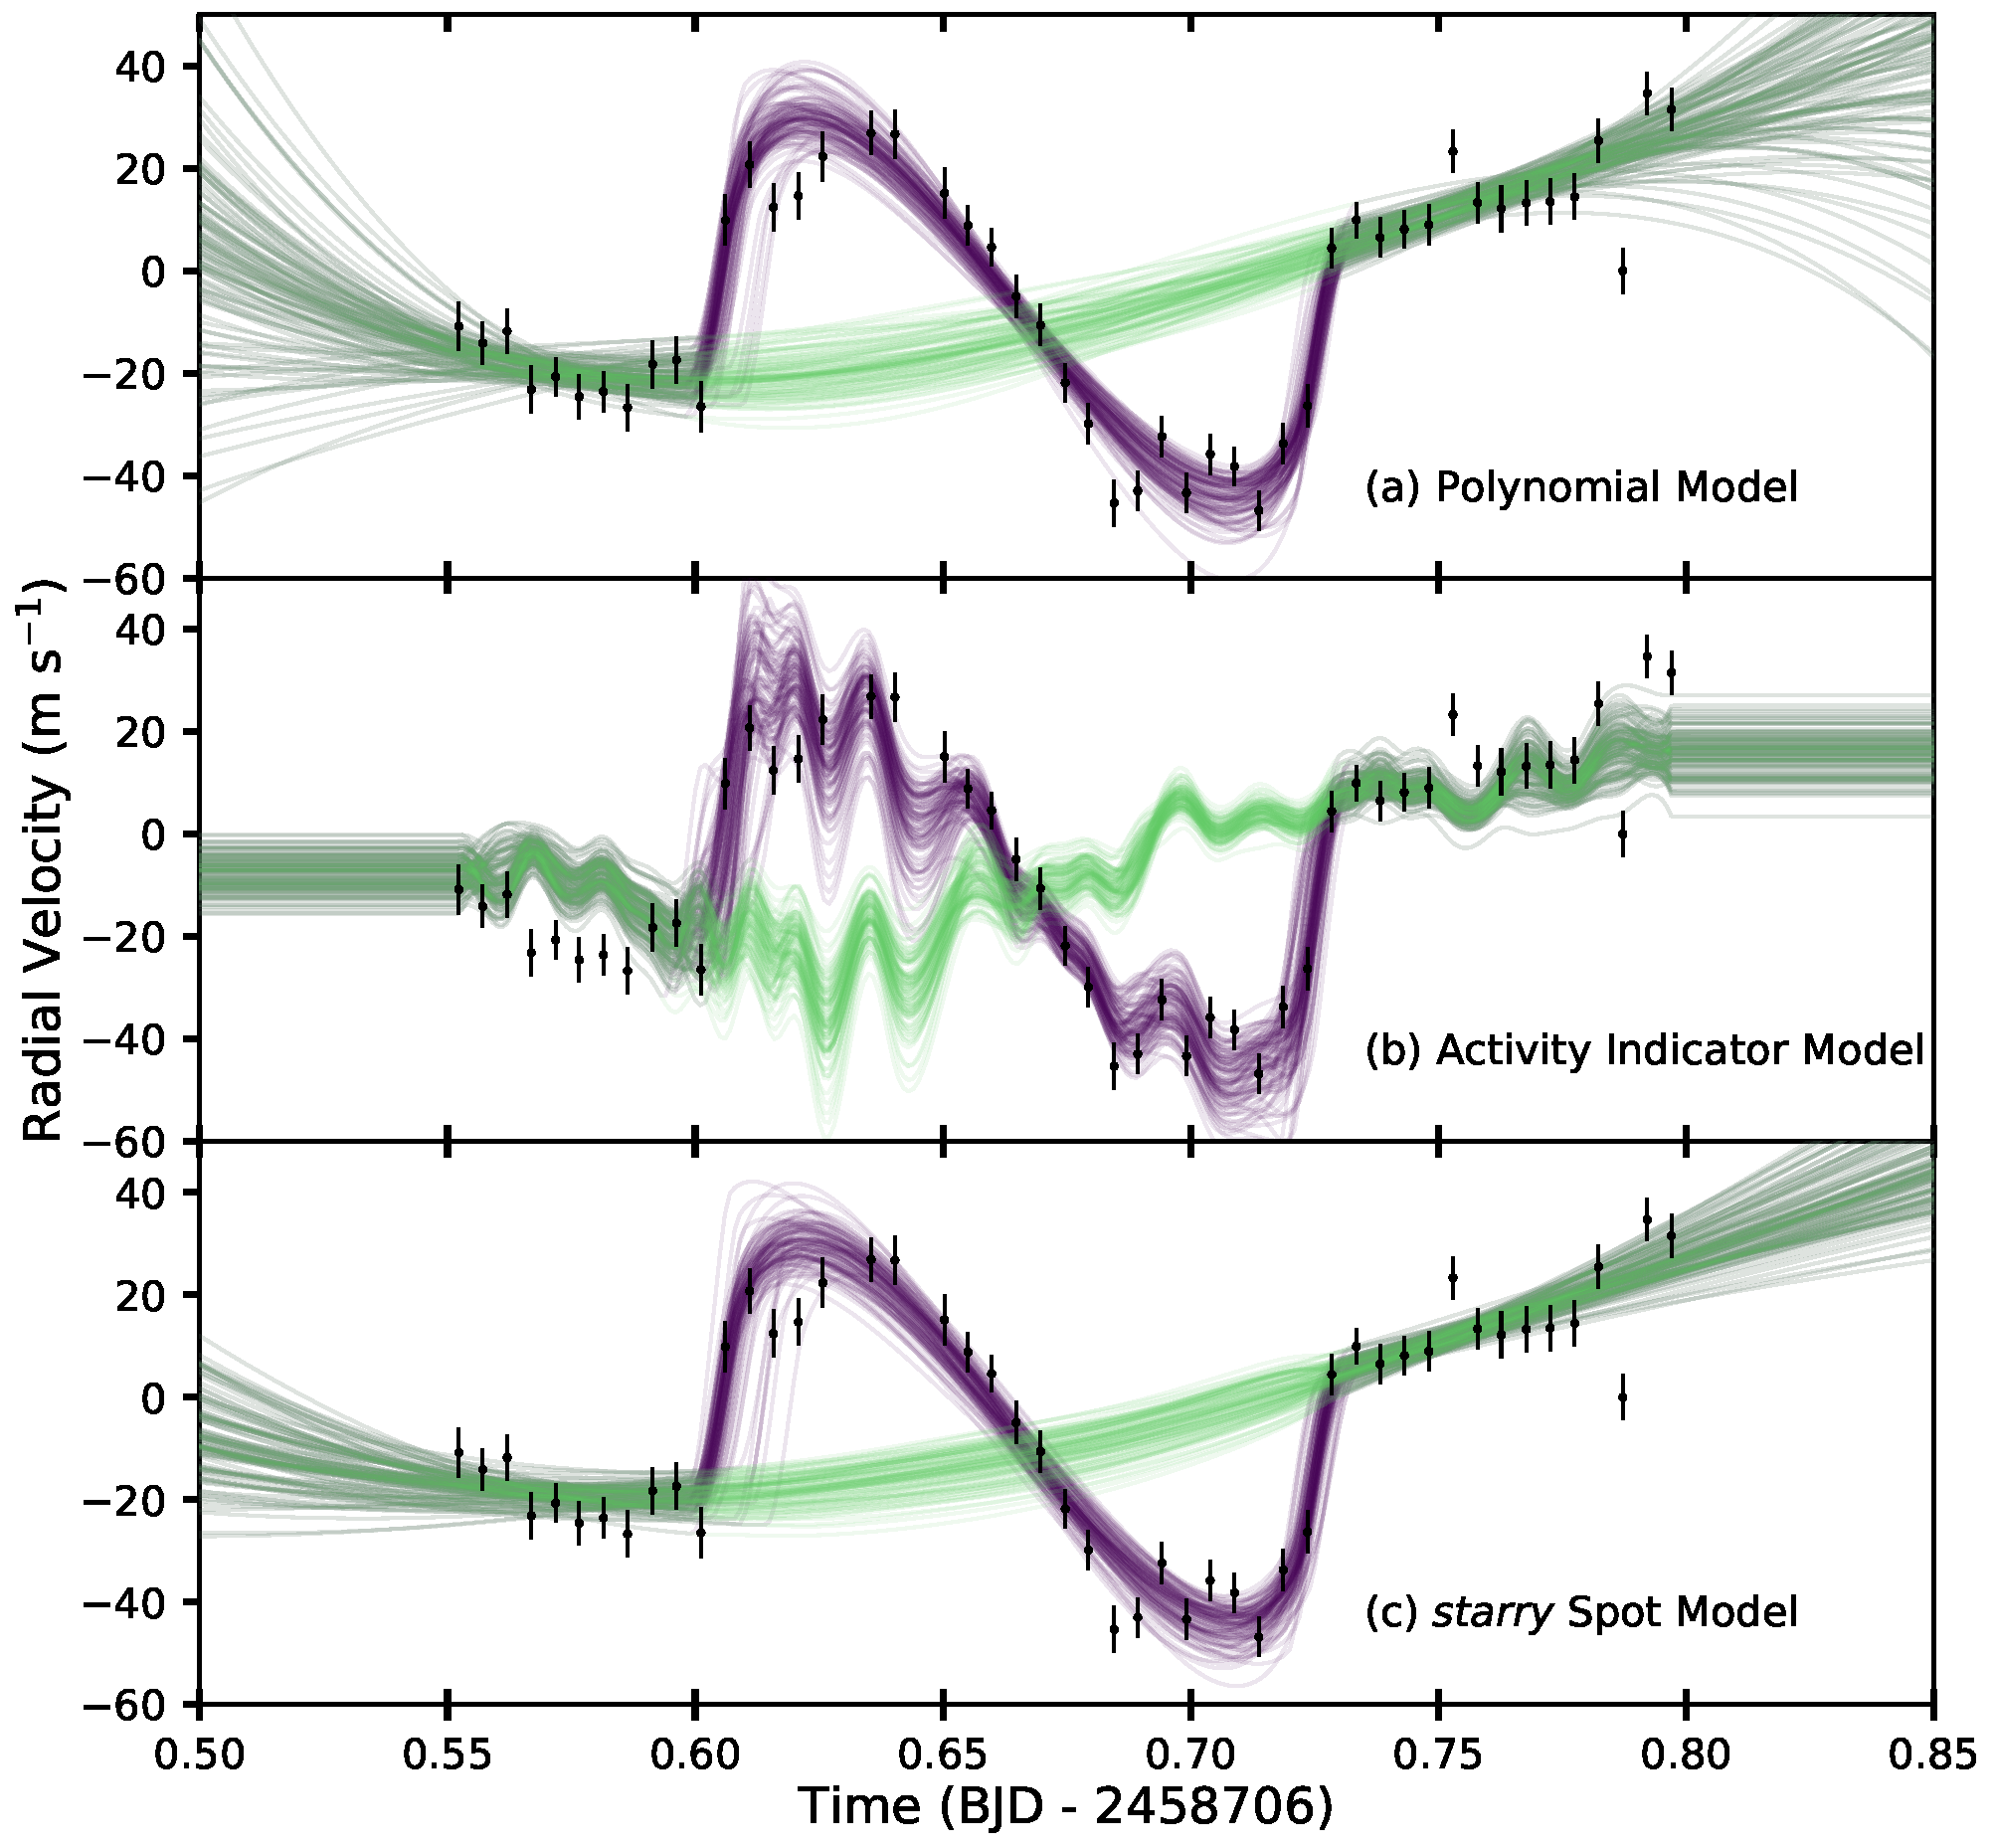
\includegraphics[width=0.45\textwidth, trim={0cm 0.0cm 1cm 1cm}, clip=true]{../figures/model_comp1.pdf}
   \end{center}
  \caption{Draws from the posterior distributions of a simultaneous fit to the
  Rossiter-McLaughlin signal and three different noise models. Green curves represent the noise model, while orange curves include the transit signal as well. From top to bottom, the noise models are a simple cubic polynomial fit, a fit regressed against the spectral stellar activity indicators, and a starspot model built with the \textit{starry} package of \citep{Luger19}. The polynomial and starspot models provide similar quality fits to the data, both of which find significantly higher log likelihood values than the third fit. Significantly, all give consistent results on the measured spin-orbit obliquity angle of approximately $12 \pm 12$ degrees.}
  \label{fig:models}
\end{figure}

\section{Discussion}
\label{sec:discussion}



Mention the fast rotation of the star, vsini of like 17 km/s? And the measured rotation period here. Wouldn't hurt to include the eleanor light curve so people can see the rotation and the magnitude of the spots, and it gets us an easy citation.

\subsection{Transit Timing}

The ephemeris from \citet{Newton19}, which includes data from both \tess\ and \spitz, predicts a transit time for this transit of $\textrm{BJD}- 2457000 = 1706.6703 \pm 0.0006$. 
The ephemeris from \citet{Benatti19}, which includes only \tess\ data, predicts a transit time of  $\textrm{BJD}- 2457000 = 1706.6903 \pm 0.0023$. 
From our data, we measure a transit time of $\textrm{BJD}- 2457000 = 1706.6654 \pm  0.0012$. 
While formally a $3\sigma$ discrepancy with each of these predictions, we note that these two predictions, using largely the same original data set, make predictions for the observed epoch which are $8\sigma$ discrepant with each other. 

While it is possible the observed variations are due to the presence of an additional nearby planet, it is also possible that these analyses underestimated their photomeric uncertainty. 
Both analyses used a Gaussian process to model the stellar rotation, but neither directly considered the effects of correlated noise on p-mode timescales on their photometry. 
As \textit{TESS} data is collected at a two-minute cadence, the five-minute p-mode oscillations are non-negligible for a solar mass and radius star \citep{Chaplin13}, and may affect the resultant precision in individual transit times.


Combining the \tess\ and \spitz\ data with our own transit time, we update the orbital period to $P= 8.13816 \pm 0.00003$ days. 
We note that we do not explicitly model the p-modes either, and if they contribute significantly to the RV variability, with one data point every seven minutes on average we may be suspect to the same underestimation.
We encourage other follow-up measurements of the transit to confirm or refute the presence of transit timing variations in this system.


\subsection{Long-term trend}

Over the six hours of the transit, the apparent RV of the star increases at approximately 10 m s$^{-1}$ hr$^{-1}$. 
In Section \ref{sec:analysis}, we model this RV shift using a toy model of a single 
starspot group moving across the surface of the star, finding this provides an appropriate fit to the data. 
However, we also use low-order polynomials to attempt to fit the data, finding that simple hueristic works approximately equally well.
This could, in principle, be caused by observing a fraction of a Keplerian orbit from another object orbiting inducing an RV shift on the star. 
We can easily rule out the wide binary companion as the culprit.
From \citet{Liu02}, the RV acceleration from a wide binary companion with mass $m$ at a known separation $\rho$ observed at a distance $d$ is always bounded such that:
\begin{equation}
    \frac{d\textrm{RV}}{dt} < 197 \textrm{m } \textrm{s}^{-1} \textrm{ d}^{-1}
    \frac{m}{M_\odot} \bigg(\frac{d}{1\textrm{pc}}\bigg)^{-2} \bigg(\frac{\rho}{1''}\bigg)^{2}.
\end{equation}
For this companion, the RV trend induced must be no more than 1 m s$^{-1}$ yr$^{-1}$, much less than the observed acceleration.

\citet{Benatti19} show the RV of DS Tuc A is stable at the $\approx 200$ m s$^{-1}$ level on decadal timescales. 
Therefore, if the trend observed during the transit were caused by a planet, it must be a planet with a period shorter than approximately 20 days. 
If this planet is external to DS Tuc Ab, then it must have $m \sin i \geq 10$ \mjup. 
\citet{Benatti19} rule out any such planets in their analysis of the system.
The only plausble planetary companion which could cause this signal but evade detection is a planet in a 1-3 day orbit with a mass of 1-3 times that of Jupiter. 

Such a companion need only be stable for a relatively short time given the age of the system; a companion similar to this one would likely induce significant TTVs which could be detected by continued transit monitoring.
However, starspot-induced modulation is a likely culprit which can explain the observed variability.


\subsection{Starspot-induced modulation}

The starspot explanation explains the data well from the night of the transit.
The toy model of Section \ref{sec:analysis} demands a starspot on the redshifted hemisphere of the star, rotating away from our line of sight during the transit. 
While we use a single, Gaussian spot in our modeling, in reality spots are non-Gaussian and often appear in groups \citep[e.g.][]{Kilcik11}.

This may explain the excess variability observed in the second half of our transit. 
Over this part of the transit, the observed point-to-point variability is larger, which may be the result of the planet crossing the relatively more inhomogenous hemisphere, causing an increase in the variability of the observed RV shift.

Our median toy model of a single spot, carried over the entire surface of the star, causes in our model a total RV variation of 235 m s$^{-1}$; the 68\% confidence interval on the peak-to-peak RV shift from this starspot ranges from 191 to 299 m s$^{-1}$.
Therefore, a single large spot group can explain both the variability observed during the night of the transit itself and the observed RV scatter on rotational timescales.
This does not mean there is only a single spot group on the surface of the star, but rather informs us about the relative asymmetries in spot coverage from hemisphere to hemisphere as the star rotates.


\subsection{Characterizing the Starspots of DS Tuc A}
The \textit{starry} model, in addition to matching the observed RV variability, also approximately matches the photometric variability observed during the \tess\ mission. 
This particular spot model induces variability at the $1.9\% \pm 0.4\%$ level.

We can compare this 


Figure \ref{fig:lc_data} shows a light curve for DS Tuc A from the \tess\ mission, built using the \btmtodo{flux} model from the \eleanor\ software package of \citet{Feinstein19}.

\begin{figure}[!tbh]
  \begin{center}
    \includegraphics[width=0.5\textwidth, trim={0cm 0.0cm 0cm 0cm}, clip=true]{../figures/lcs1.pdf}
   \end{center}
  \caption{(Left) DS Tuc A light curve from the \tess\ Sector 1 Full-Frame Images, built with the \eleanor\ pipeline of \citet{Feinstein19}. (Right) ASAS-SN light curve for the same star, with the \tess\ light curve overlaid in green. While \tess\ shows a 4\% variability on rotational timescales, the star itself varies on multi-year timescales by as much as 30\%, suggesting significant starspot coverage on the stellar surface. The brightest cadences observed with \tess\ are approximately 10\% fainter than the brightest observations with ASAS-SN.}
  \label{fig:lc_data}
\end{figure}

\btmtodo{more}


\subsection{The Power of Obliquity Measurements of Young Stars}

We have seen from these data that the RV of DS Tuc A varies by nearly 300 m s$^{-1}$ on rotational timescales. 
However, because the surface is relatively consistent on transit timescales, the R-M signal is relatively easy to disentangle from the rotational modulation despite being an order of magnitude smaller in amplitude.

Recent work has shown the potential to measure orbits of planets in the face of extreme stellar activity \citep{Barragan19}, and this still remains the only feasible way to measure masses of transiting planets spectroscopically. 
However, even without a mass we are able to confirm this planet which had only been statistically validated in previous works. 
From the R-M detection, we can be sure this event is the result of an object transiting the surface of DS Tuc A. 
As the transit depth from \tess\ precludes the possibility this event is caused by a transiting brown dwarf or low-mass star, the only possible cause for this observed event is a bona fide transiting planet.
DS Tuc Ab thus joins a small number of planets that have been confirmed through the secure detection of their R-M signal, and is the first member of this class discovered by the \tess\ mission \citep{Jenkins10b, Hirano12b}. 

DS Tuc A has a measured \vsini of \btmtodo{number}, meaning it is not amenable to precision RV work.
More massive stars which lack convective outer layers can rotate at similar speeds \btmtodo{cite}.

Bigger signal than RVs here. --- future confirmation for young systems!


\btmtodo{say something about getting a template on the same night as the transit.}

\subsubsection{Differential Rotation}



cite \citet{Giminez06} in this section probably.


Differential rotation not measureable unless system highly misaligned. Even then the signal is smaller than the scatter due to starspots (1 m/s for a system like this one) so many observations at high SNR will be required to disentangle. This is going to be tough!

Could we say something about differential rotation from multiple planets? This seems at odds with the previous graph. Maybe in idealized cases? Need to work through this consideration!


Somewhere: \citet{Oshagh18} on limitations of R-M for very active stars.


\subsection{Conclusions}



\acknowledgements

We thank \btmtodo{people including George Zhou and Leslie Rogers} for \btmtodo{things}.

This paper includes data gathered with the 6.5 meter Magellan Telescopes located at Las Campanas Observatory, Chile.


This research was enabled by the Exostar19 program at the Kavli Institute for Theoretical Physics at UC Santa Barbara, which was supported in part by the National Science Foundation under Grant No. NSF PHY-1748958.

This project was developed in part at the \textit{Building Early Science with} TESS meeting, which took place in 2019 March at the University of Chicago.

Work by B.T.M. was performed in part under contract with the Jet
Propulsion Laboratory (JPL) funded by NASA through
the Sagan Fellowship Program executed by the NASA
Exoplanet Science Institute.

This material is based upon work supported by the National Science Foundation Graduate Research Fellowship Program under Grant No. (DGE-1746045). Any opinions, findings, and conclusions or recommendations expressed in this material are those of the author(s) and do not necessarily reflect the views of the National Science Foundation.



This paper includes data collected by the TESS mission. Funding for the TESS mission is provided by the NASA Explorer Program.

TESS data were obtained from the Mikulski Archive for Space Telescopes
(MAST).
STScI is operated by the Association of Universities for Research in
Astronomy, Inc., under NASA contract NAS5-26555.
Support for MAST is provided by the NASA Office of Space Science via grant
NNX13AC07G and by other grants and contracts.



\software{%
    numpy \citep{numpy},
    matplotlib \citep{matplotlib},
    scipy \citep{Jones01}
    astropy \citep{Astropy18},
    eleanor \citep{Feinstein19},
    starry \citep{Luger19},
    emcee \citep{Foreman-Mackey12}
    }

\facility{Magellan:Clay (Planet Finder Spectrograph), TESS}





\bibliography{exopapers}






\end{document}


